\chapter{പെണ്ണരശുനാടോ? കേരളമോ?}
\label{chapter2}  

\begin{figure}[h]
\begin{center}
\includegraphics[width=\textwidth,height=10cm]{Kulasthree_Chapter02_pic01.jpg}
\end{center}
\end{figure}

\textit{\paragraph{}
 മരുമക്കത്തായികളായിരുന്ന മലയാളികൾക്കിടയിൽ സ്ത്രീകൾ വളരെ സ്വതന്ത്രരായിരുന്നുവെന്ന അവകാശവാദം നാം സാധാരണ കേൾക്കാറുള്ളതാണ്. വിവാഹം, സ്വത്തവകാശം എന്നീ രണ്ടുകാര്യങ്ങളിൽ മരുമക്കത്തായം പിന്തുടർന്നിരുന്ന സമുദായങ്ങളിലെ സ്ത്രീകൾക്ക് ആനുകൂല്യമുണ്ടായിരുന്നുവെന്ന് നമുക്കറിയാം. എന്നാൽ ഇതുകൊണ്ടുമാത്രം കേരളം 'പെണ്ണരശുനാടാ'യിരുന്നുവെന്ന് പറയാനൊക്കുമോ? ദൈനംദിനജീവിതത്തിന്റെ ഭാരം മേലാളസ്ത്രീകൾക്ക് കുറവായിരുന്നോ? മാത്രമല്ല, വരേണ്യസ്ത്രീകളുടെ അനുഭവത്തെമാത്രം കണക്കാക്കുന്ന രീതി തീർച്ചയായും ചരിത്രരചനയിൽ ആശാസ്യമല്ല. കീഴാളസ്ത്രീകളുടെ അനുഭവങ്ങൾകൂടി കണക്കാക്കിയാൽ 'സ്ത്രീസ്വാതന്ത്ര്യ'ത്തെ പരമ്പരാഗതമായി പോഷിപ്പിച്ച സമൂഹം' എന്ന പേരിന് നാം അർഹരല്ലെന്നു കാണാം.}
 
 \section{'ജന്മഭേദവ്യവസ്ഥ'യിലെ സ്ത്രീകൾ}


\paragraph{}'സ്ത്രീകൾ ഭരിക്കുന്ന നാട്' എന്ന് ഇന്ന് കേരളത്തെ ആരെങ്കിലും വിശേഷിപ്പിച്ചാൽ ആ വ്യക്തിക്ക് തീരെ അറിവില്ലെന്നേ നാം വിചാരിക്കൂ. പക്ഷേ പണ്ട്, അതായത് പത്തൊമ്പതാം നൂറ്റാണ്ടിൽ, കേരളത്തിന് 'പെണ്ണരശുനാട്' അഥവാ 'പെൺഭരണം നിലവിലുള്ള നാട്' എന്നു പേരുണ്ടായിരുന്നു. മരുമക്കത്തായ കുടുംബരീതികൾ സ്ത്രീകൾക്കനുവദിച്ചിരുന്ന ചില തെരഞ്ഞെടുപ്പുകളെക്കുറിച്ചായിരിക്കാം ഇതു സൂചിപ്പിക്കുന്നത്. മരുമക്കത്തായ കുടുംബവ്യവസ്ഥയിൽ ചില ഘടകങ്ങൾ സ്ത്രീകൾക്കനുകൂലമായിരുന്നുവെന്ന വസ്തുത ഇന്ന് പരക്കെ അംഗീകരിക്കപ്പെടുന്നുണ്ട്. എന്നുവച്ച് മരുമക്കത്തായികളായ സ്ത്രീകൾ 'സർവ്വസ്വതന്ത്രകൾ' ആയിരുന്നില്ലെന്നു നമുക്കറിയാം. മരുമക്കത്തായത്തിൽ - അതായത് സ്വത്തവകാശം ഒരു തലമുറയിൽനിന്ന് അടുത്തതലമുറയിലേക്ക് നീങ്ങുന്നത് പെൺവഴിക്കായിരുന്ന രീതിയിൽ - സ്ത്രീകൾക്ക് കൂടുതൽ നിലയും വിലയുമുണ്ടായത് സ്വാഭാവികംമാത്രം. കാരണം, കുടുംബം തുടരുന്നത് പെണ്മക്കളുടെ മക്കളിലൂടെയാകുമ്പോൾ മകൾക്ക് ഒരുവിധം നല്ല പരിഗണന കൊടുത്തല്ലേ പറ്റൂ?

\paragraph{}മലയാളികൾ എല്ലാവരും മരുമക്കത്തായികളായിരുന്നില്ലെന്ന് ഓർക്കേണ്ടതുണ്ട്. കുടുംബത്തിന്റെ പിന്തുടർച്ച ആൺമക്കളിലൂടെ കണക്കാക്കിയിരുന്ന മക്കത്തായവ്യവസ്ഥ പിന്തുടർന്നവരും (ഉദാഹരണത്തിന്, സുറിയാനി ക്രിസ്ത്യാനികൾ, നമ്പൂതിരിമാർ) മക്കത്തായ-മരുമക്കത്തായവ്യവസ്ഥകളെ കൂട്ടിയിണക്കി 'മിശ്രദായം' അംഗീകരിച്ചിരുന്നവരും (ഉദാഹരണത്തിന് ഈഴവരിൽ ചില വിഭാഗക്കാർ) ഇവിടെയുണ്ടായിരുന്നു. ഇക്കൂട്ടർക്കിടയിൽ സ്ത്രീകൾക്ക് ഔപചാരികനിലയിൽ ഒരുപാട് അധികാരമുണ്ടായിരുന്നുവെന്ന് പറയാൻ കഴിയില്ല. അതുകൊണ്ട് കേരളത്തെ ഒന്നടങ്കം 'പെണ്ണരശുനാടെ'ന്ന് വിശേഷിപ്പിച്ചത് ശരിതന്നെയോ എന്ന ചോദ്യം പ്രസക്തമാണ്. കേരളത്തിലെ എല്ലാ സ്ത്രീകൾക്കും ഒരുപോലെ ബാധകമായ ഒരു സ്ത്രീസങ്കല്പം, അല്ലെങ്കിൽ സ്ത്രീത്വാദർശം, പരമ്പരാഗത മലയാളിസമൂഹത്തിൽ ഉണ്ടായിരുന്നില്ലെന്നു പറയാം. പരമ്പരാഗത കേരളീയ സമൂഹത്തെ 'ജന്മഭേദവ്യവസ്ഥ' എന്നു നമുക്കു വിളിക്കാം. ഒരു വ്യക്തി ഏതു ജാതിവിഭാഗത്തിൽ ജനിക്കുന്നുവോ, ആ വിഭാഗത്തിന്റെ പൊതുനിയമങ്ങൾക്ക് അടിപ്പെട്ട് ജീവിതകാലം മുഴുവൻ കഴിച്ചുകൂട്ടിക്കൊള്ളണമെന്ന നിബന്ധന ഇതിന്റെ അടിസ്ഥാനപ്രമാണങ്ങളിലൊന്നായിരുന്നു.


\paragraph{}ഒരു ജാതിയിൽ ജനിച്ചാൽ മറ്റൊരു ജാതിയിലേക്കു മാറാൻ മിക്കപ്പോഴും കഴിയില്ലായിരുന്നു; ജനിക്കുന്ന ജാതിയുടെ നിയമങ്ങൾ തെറ്റി നടന്നാൽ ജാതിയിൽനിന്ന് പുറന്തള്ളൽ അഥവാ ഭ്രഷ്ട് എന്ന ശിക്ഷ ലഭിക്കാൻ സാദ്ധ്യതയുമുണ്ടായിരുന്നു. ജാതിവ്യവസ്ഥ ഒരു ഉച്ചനീചത്വശ്രണിയായിരുന്നതുകൊണ്ടുതന്നെ, 'മുകളിലെ' ജാതിക്കാർക്ക് കീഴ്‌വഴങ്ങി 'കീഴിലു'ള്ളവർ കഴിഞ്ഞുകൊള്ളണമെന്നായിരുന്നു നിയമം. കീഴ്ജാതിക്കാരുടെ അധമനില സൂചിപ്പിക്കാനുള്ള ചിഹ്നങ്ങൾ ദൈനംദിനജീവിതത്തിലും ഭാഷയിലും ജീവിതത്തിന്റെ സമസ്തമേഖലകളിലും നിറഞ്ഞുനിന്നിരുന്നു.

%%%%%BOX%%%%%%
\captionof{mybox}{ബ്രാഹ്മണപിതൃമേധാവിത്വം}\label{ch2box1} % place the caption
\begin{tcolorbox}[%
  breakable, % make the box breakable
  arc=0mm, 
  left=1pt, right = 1pt, 
  boxrule=0mm,
  colback = {blue!10}, % since shadow-gray was not defined
] 

{\begin{center}
\includegraphics[width=0.4\textwidth,height=4cm]{Kulasthree_Chapter02_pic02.jpg}
\end{center}
\paragraph{}ഇന്ത്യയിലെ സ്ത്രീചരിത്രരചനാരംഗത്തെ ഏറ്റവും പ്രധാനപ്പെട്ട നാമങ്ങളിലൊന്നാണ് ദില്ലി സർവ്വകലാശാലയിൽ പ്രവർത്തിച്ചിരുന്ന ചരിത്രകാരിയായ ഉമാ ചക്രവർത്തിയുടേത്. ഇന്ത്യൻ സമൂഹത്തിൽ ജാതിവ്യവസ്ഥയും സ്ത്രീകളുടെമേൽ നടപ്പിലുള്ള നിയന്ത്രണങ്ങളും തമ്മിലുള്ള അഭേദ്യബന്ധത്തെ സൂക്ഷ്മമായി അപഗ്രഥിക്കുന്നവയാണ് അവരുടെ ചരിത്രപഠനങ്ങൾ. പരമ്പരാഗത ഇന്ത്യൻ സമൂഹത്തിൽ നിലനിന്നിരുന്ന ആൺകോയ്മയെ 'ബ്രാഹ്മണപിതൃമേധാവിത്വം' (brahmanical patriarchy) എന്നാണ് അവർ വിളിക്കുന്നത്. ഇതുപ്രകാരം ഉയർന്ന ജാതികളിൽപ്പെട്ട സ്ത്രീകളെ മേലാളജാതികളുടെ പ്രജനനത്തിനുള്ള ഉപകരണങ്ങളായി കരുതുന്നു. കീഴ്ജാതിസ്ത്രീകളെ ഉയർന്ന ജാതിക്കാർക്കുവേണ്ടി അദ്ധ്വാനിക്കാനും അവരുടെ ലൈംഗികാവശ്യങ്ങൾ നിവർത്തിക്കുന്നതിനായും നിയോഗിക്കുന്നു. ജാതിവ്യവസ്ഥയെ സംരക്ഷിക്കുന്നതിന് മേൽജാതി സ്ത്രീകളെ സമൂഹത്തിൽനിന്ന് ഒഴിച്ചുനിർത്തേണ്ടത് ആവശ്യമാണെന്ന് 'ബ്രാഹ്മണപിതൃമേധാവിത്വ'ത്തിന്റെ വക്താക്കൾ എക്കാലത്തും വാദിച്ചിട്ടുണ്ട്. അന്യജാതിക്കാരുമായി, പ്രത്യേകിച്ച് കീഴ്ജാതിക്കാരായ പുരുഷന്മാരുമായി, അവർ സംസർഗ്ഗത്തിലേർപ്പെട്ടാൽ ഉയർന്നജാതിയുടെ അടിത്തറതന്നെ തകർന്നുപോകുമെന്നുള്ളതുകൊണ്ടാണ് അവരുടെമേൽ വളരെ കടുത്ത നിയന്ത്രണങ്ങൾ ഏർപ്പെടുത്തിയിരുന്നത്. ബ്രാഹ്മണ നിയമവ്യവസ്ഥയും ഇവിടുത്തെ രാജഭരണവും മേൽജാതി സ്ത്രീകൾക്കുമേലുള്ള നിയന്ത്രണങ്ങളെ ന്യായീകരിച്ചു. ആ നിയന്ത്രണങ്ങളെ എതിർത്ത, അല്ലെങ്കിൽ ലംഘിച്ച സ്ത്രീകളെ പുറന്തള്ളാൻ മേൽജാതി സമുദായങ്ങൾ തീരെ മടിച്ചിരുന്നില്ല.}
\end{tcolorbox}
%%%%%%%%%%%

\begin{figure}[h]
\begin{center}
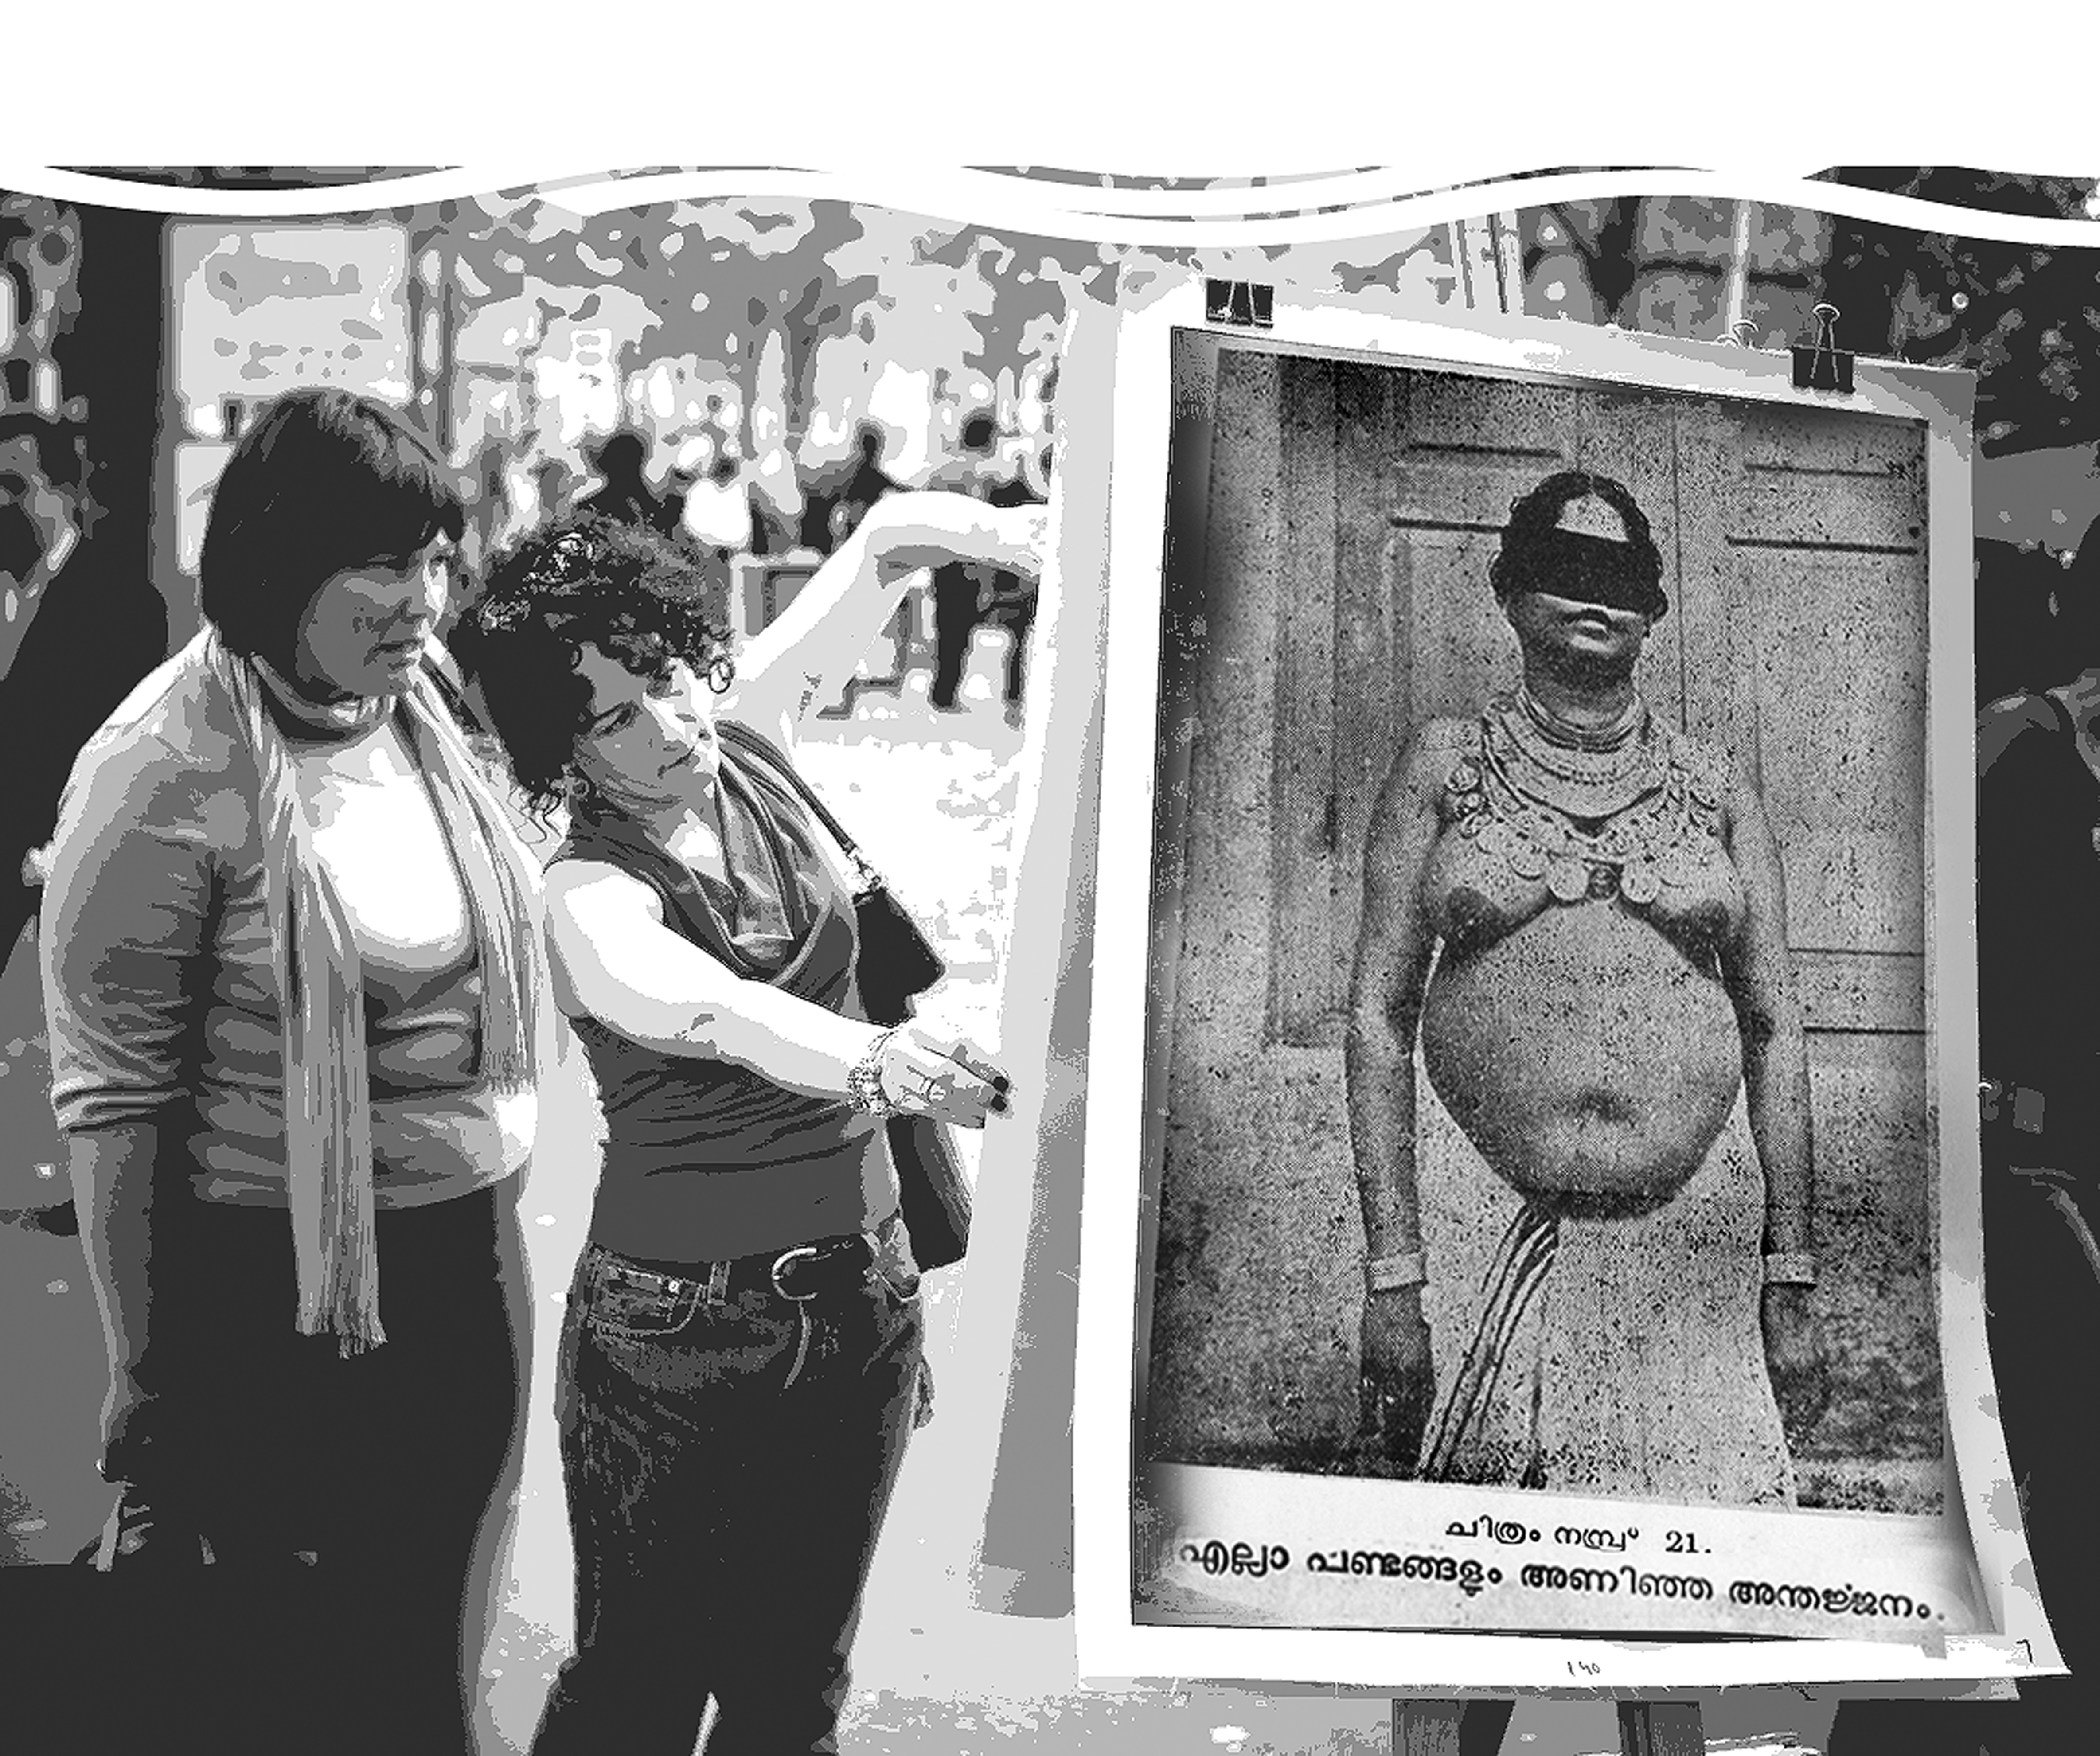
\includegraphics[width=\textwidth,height=8cm]{Kulasthree_Chapter02_pic03.jpg}
\end{center}
\end{figure}

\paragraph{}'ജന്മഭേദവ്യവസ്ഥ'പ്രകാരം ഓരോ ജാതിയിലേയും ആണുങ്ങൾക്കും പെണ്ണുങ്ങൾക്കും വെവ്വേറെ ലിംഗനിയമങ്ങളുണ്ടായിരുന്നു. അതായത് മലയാളബ്രാഹ്മണ (നമ്പൂതിരി) സമുദായത്തിലെ 'ഉത്തമസ്ത്രീസങ്കല്പം' നായർസ്ത്രീകൾക്കോ കീഴ്ജാതിക്കാർക്കോ ബാധകമായിരുന്നില്ല. ഓരോ സമുദായത്തിനും ഇതൊക്കെ പ്രത്യേകം പ്രത്യേകമുണ്ടായിരുന്നു. തീർച്ചയായും അന്നുള്ളവർ ധാരാളം വായിച്ചിരുന്ന പുരാണങ്ങളിലൂടെയും ശീലാവതിചരിതംപോലുള്ള കൃതികളിലൂടെയും ബ്രാഹ്മണരുടെ ലിംഗമൂല്യങ്ങൾ (അതായത്, ആണുങ്ങളായാൽ എങ്ങനെയിരിക്കണം, എന്തു ചെയ്യണം എന്നും പെണ്ണുങ്ങളായാൽ എങ്ങനെയിരിക്കണം, എന്തു ചെയ്യണം എന്നും മറ്റും വിധിക്കുന്ന മൂല്യങ്ങൾ) സമൂഹത്തിൽ പ്രചരിച്ചിരുന്നു. എന്നാൽ, ഇതോടൊപ്പംതന്നെ ഈ മൂല്യങ്ങൾ എല്ലാ സ്ത്രീകൾക്കും ബാധകമല്ലെന്നു സ്ഥാപിക്കുന്ന 'ബ്രാഹ്മണന്യായീകരണങ്ങ'ളും പ്രചരിച്ചിരുന്നുവെന്ന് കാണേണ്ടതുണ്ട്. ഉദാഹരണത്തിന്, കേരളത്തിലെ ശൂദ്രസ്ത്രീകൾ (നായർ-അമ്പലവാസി സമുദായക്കാർ) പാതിവ്രത്യം ആചരിക്കേണ്ടതില്ലെന്ന് കേരളമാഹാത്മ്യം പോലുള്ള ഗ്രന്ഥങ്ങൾ ഉദ്ധരിച്ചുകൊണ്ട് പഴമക്കാർ വാദിച്ചിരുന്നു - ഇവിടത്തെ ശൂദ്രസ്ത്രീകൾ ദേവന്മാരെ ആനന്ദിപ്പിക്കുന്നതിനായി സൃഷ്ടിക്കപ്പെട്ട അപ്സരസ്സുകളുടെ സന്തതികളാണെന്നും അപ്സരസ്ത്രീകൾക്ക് പാതിവ്രത്യം ബാധകമല്ലാത്തതുപോലെ അവരുടെ സന്തതികൾക്കും അതു ബാധകമല്ലെന്നും ഈ കൃതികൾ പറയുന്നു. അതുകൊണ്ട് ശീലാവതിചരിതം വായിച്ചു പുണ്യംസമ്പാദിച്ച നായർസ്ത്രീകൾ ശീലാവതിയെ മാതൃകയാക്കിക്കളയുമെന്ന് പ്രതീക്ഷിക്കേണ്ടതില്ലായിരുന്നു! അതേസമയം ജാതികൾ തമ്മിൽ ലിംഗമൂല്യങ്ങളിൽ കാര്യമായ വ്യത്യാസമുള്ളിടത്ത് ഇവ പലപ്പോഴും വഴക്കിനും കലഹത്തിനും കാരണമായി. ഉദാഹരണത്തിന് തിരുവിതാംകൂറിലെ കരുനാഗപ്പള്ളി-കാർത്തികപ്പള്ളി മേഖലയിൽ (ഓണാട്ടുകരയിൽ) 19-ാം നൂറ്റാണ്ടിൽ നടന്ന ജാതീയ ഏറ്റുമുട്ടലുകളെക്കുറിച്ച് വാമൊഴിയായി പ്രചരിച്ചിട്ടുള്ള കഥകളിൽ പലതിലും വിഷയം മേൽപ്പറഞ്ഞ ലിംഗമൂല്യങ്ങളിലെ പൊരുത്തക്കേടാണ്. മുസ്ലിം സമുദായത്തിലെ സമ്പ്രദായപ്രകാരം സ്ത്രീകൾ നിർബന്ധമായും മേൽവസ്ത്രം ധരിച്ചിരിക്കണം; ഈഴവരുടെയിടയിൽ അക്കാലത്ത് നേരെ തിരിച്ചായിരുന്നു നിയമം - അതായത്, മേൽവസ്ത്രം ധരിച്ചുനടക്കുന്നത് 'നല്ല സ്ത്രീകൾ' ചെയ്യുന്ന പണിയല്ല, 'വേഷംകെട്ടുകാരത്തികളു'ടെ പണിയാണ്! ഈ പ്രദേശത്തെ ചന്തകളിൽ കച്ചവടക്കാര്യത്തിലുംമറ്റും ഈ രണ്ടു സമുദായക്കാർ തമ്മിൽ കടുത്ത മത്സരം നിലനിന്നിരുന്നതുകൊണ്ട് അടികലശലിനുംമറ്റും സാദ്ധ്യതയും കൂടുതലായിരുന്നു. പക്ഷേ, അടി പൊട്ടിപ്പുറപ്പെട്ടത് പലപ്പോഴും വസ്ത്രധാരണത്തെക്കുറിച്ചുള്ള അഭിപ്രായവ്യത്യാസങ്ങളെ ചുറ്റിപ്പറ്റിയായിരുന്നെന്ന് വാമൊഴിക്കഥകൾ സൂചിപ്പിക്കുന്നു. നഗ്നമായ മാറിടവുമായി ചന്തയിലെത്തിയിരുന്ന ഈഴവസ്ത്രീകളെ മുസ്ലീം പുരുഷന്മാർ കളിയാക്കിയെന്നും തുടർന്നു ലഹളയുണ്ടായെന്നുംമറ്റുമാണ് കഥകളിലെ പരാമർശം.


\paragraph{}'ജാതിയിൽ കൂടിയ സ്ത്രീകൾക്ക് കൂടിയ സ്വാതന്ത്ര്യം' എന്ന ഇന്നത്തെക്കണക്ക് അന്ന് എല്ലായിടത്തും ഒത്തിരുന്നില്ലെന്നതാണ് രസകരമായ വസ്തുത. ജാതിയിൽ ഏറ്റവും മുന്തിയവർ എന്ന് സ്വയം അവകാശപ്പെട്ട ബ്രാഹ്മണസ്ത്രീകൾ അതികഠിനമായ നിയന്ത്രണങ്ങൾക്കു വിധേയരായിരുന്നു. അതേസമയം 'താരതമ്യേന സ്വതന്ത്രകൾ' എന്നു നാം തിരിച്ചറിയുന്ന മരുമക്കത്തായ സ്ത്രീകൾ - വിശേഷിച്ചും ഉയർന്ന ജാതിക്കാർ - മറ്റു പലവിധ നിയന്ത്രണങ്ങൾക്കുമുള്ളിലായിരുന്നു. വീട്ടിലെ അദ്ധ്വാനത്തിന്റെ കാര്യമെടുത്താൽ ഉന്നതജാതിക്കാരായ സ്ത്രീകൾപോലും അതിൽനിന്ന് പൂർണ്ണമായും ഒഴിവായിരുന്നില്ലെന്നു വ്യക്തം.

\section{വരേണ്യ മലയാളിസ്ത്രീകളുടെ ദൈനംദിനജീവിതം}
പരമ്പരാഗത മലയാളിസമൂഹത്തിൽ പല ജാതിവിഭാഗങ്ങളിൽപ്പെട്ട സ്ത്രീകളുടെയും സ്ത്രീത്വാദർശവും അവർക്കു ബാധകമായ ദൈനംദിനജീവിതനിയമങ്ങളും വെവ്വേറെയായിരുന്നെന്ന് പറഞ്ഞുവല്ലോ. ഈ വ്യത്യാസത്തിന് ഊന്നൽ നല്കിക്കൊണ്ട്, ലഭ്യമായ വിവരങ്ങൾ അനുവദിക്കുന്നിടത്തോളം പരമ്പരാഗത മലയാളിസമൂഹത്തിലെ പല ജാതിക്കാരായ സ്ത്രീകളുടെ ദൈനംദിനജീവിതം എങ്ങനെയായിരുന്നുവെന്ന് പരിശോധിക്കാനാണ് ഇവിടെ ശ്രമിക്കുന്നത്. എല്ലാ ജാതിക്കാരെക്കുറിച്ചും പറയാൻ സ്ഥലപരിമിതിയും വിവരങ്ങളുടെ കുറവും അനുവദിക്കുന്നില്ല. കേരളത്തിലെ ജാതികളുടെ ആചാരങ്ങൾ, അനുഷ്ഠാനങ്ങൾ, വിവാഹരീതി, വിവാഹകർമ്മം മുതലായവയെക്കുറിച്ച് ധാരാളം വിവരങ്ങൾ നരവംശശാസ്ത്രകൃതികളിൽനിന്നും സർക്കാരിന്റെ ഔദ്യോഗികപ്രസിദ്ധീകരണങ്ങളിൽനിന്നും ലഭ്യമാണ്. ആ വിവരങ്ങൾ ഇവിടെ ആവർത്തിക്കുന്നില്ല.
പരമ്പരാഗത മലയാളിസമൂഹത്തിൽ മേധാവിത്വമുണ്ടായിരുന്ന മലയാള ബ്രാഹ്മണരിൽനിന്നു തുടങ്ങാം. സ്ത്രീകളുടെമേൽ ഏറ്റവും ശക്തമായ നിയന്ത്രണങ്ങൾ ഏർപ്പെടുത്തിയിരുന്ന സമുദായമായിരുന്നു ഇത്. ആൺവഴിക്ക് കുടുംബപിന്തുടർച്ചയും സ്വത്തവകാശവും കണക്കാക്കിയിരുന്നതിനാൽ സ്ത്രീകൾക്ക് കാര്യമായി വിലകൽപിക്കാതിരുന്ന സമൂഹം (എങ്കിലും ഇന്ന് വടക്കേയിന്ത്യയിൽ കാണുന്നത്ര സ്ത്രീവിരുദ്ധത ഇക്കൂട്ടർക്കിടയിൽ ഇല്ലായിരുന്നെന്ന് കരുതാൻ നമ്മെ അനുവദിക്കുന്ന ചില സൂചനകളുണ്ട്). നമ്പൂതിരിയില്ലങ്ങളിൽ ജനനംമുതൽക്കേ ആൺകുട്ടിക്ക് പ്രത്യേക പരിഗണന നൽകുന്ന പല സമ്പ്രദായങ്ങളും പിന്തുടർന്നിരുന്നുവെന്ന് നമ്പൂതിരിസമുദായത്തെക്കുറിച്ച് എഴുതിയ കാണിപ്പയ്യൂർ ശങ്കരൻ നമ്പൂതിരിപ്പാട് പറയുന്നു. പ്രായപൂർത്തിയായിക്കഴിഞ്ഞാൽ പെൺകുട്ടി അന്യപുരുഷന്മാരുമായി സംസാരിച്ചുകൂടാ; എട്ടു വയസ്സുകഴിഞ്ഞാൽ അവൾ വീട്ടുജോലി ചെയ്തുതുടങ്ങണം; കന്യകമാർ നല്ല ഭർത്താവിനെ ലഭിക്കാൻ കഠിനമായ വ്രതങ്ങൾ നോക്കണം - ഇങ്ങനെയൊക്കെയായിരുന്നു നിയമങ്ങൾ. ചേലപ്പുതപ്പുകൊണ്ട് ഉടലാകെ മൂടി, വലിയ മറക്കുടചൂടി, വേലക്കാരുടെ അകമ്പടിയോടെമാത്രമേ നമ്പൂതിരിസ്ത്രീകൾക്ക് (അക്കാലത്ത് മലയാളബ്രാഹ്മണസ്ത്രീകളെ 'അന്തർജനങ്ങൾ' എന്നാണ് വിളിച്ചിരുന്നത്) ഇല്ലംവിട്ട് സഞ്ചരിക്കാൻ അനുവാദമുണ്ടായിരുന്നുള്ളൂ.

\paragraph{}'ഉപനയനം' എന്ന ചടങ്ങുകഴിഞ്ഞാൽ നമ്പൂതിരിബാലന്മാരുടെ ജീവിതവും ദുഃസഹമായിരുന്നെന്ന സൂചന അക്കാലത്തു ജീവിച്ചിരുന്ന പലരുടെയും ആത്മകഥകളിലുണ്ട്. പക്ഷേ, ഈ കഷ്ടപ്പാടിലൂടെ കടന്നുകഴിഞ്ഞാൽ സമുദായത്തിൽ പൂർണ്ണമായ അംഗത്വവും അധികാരവും അവർക്ക് ലഭിക്കുമായിരുന്നു. വാരം, പൂരം തുടങ്ങിയ വിശേഷാവസരങ്ങളിൽ അമ്പലങ്ങളിലും മറ്റു നമ്പൂതിരിയില്ലങ്ങളിലും ഒത്തുകൂടി സദ്യയും വെടിവട്ടവുമായി കഴിയാൻ അവർക്കു കഴിയുമായിരുന്നു. കഷ്ടിച്ച് വായിക്കാൻ പഠിച്ചാൽ അന്തർജനത്തിന്റെ വിദ്യാഭ്യാസം കഴിയും; പിന്നെ വീട്ടിനുള്ളിലും പരിസരത്തുള്ള ഇല്ലങ്ങൾ, അമ്പലങ്ങൾ എന്നിവിടങ്ങളിലും സ്വന്തം വീട്ടിലും മാത്രമായി അവരുടെ ജീവിതം കഴിയും.

\paragraph{}ഇല്ലങ്ങളിലെ അന്തർജനങ്ങളുടെ ദിനചര്യ വളരെ കൃത്യമായി ആവർത്തിക്കേണ്ട ചടങ്ങുകളുടെ നീണ്ട ശൃംഖലതന്നെയായിരുന്നുവെന്നു പറയാം. കുളിപോലും സൂക്ഷിച്ചു ചെയ്യേണ്ട ചടങ്ങുകളുടെ കൂട്ടമായിരുന്നുവെന്ന് കാണിപ്പയ്യൂരിന്റെ വിവരണം വ്യക്തമാക്കുന്നു. അന്തർജനങ്ങൾക്കിടയിൽത്തന്നെ അവിവാഹിതകളായ പെൺകുട്ടികളും വിധവകളുമായിരുന്നു കഠിനവ്രതങ്ങൾ അനുഷ്ഠിച്ചിരുന്നത് - വിധവയെ സംബന്ധിച്ചിടത്തോളം ഭർത്താവിന്റെ മരണശേഷമുള്ള ജീവിതം നീണ്ട ഒരു പ്രായശ്ചിത്തമെന്നോണം ചെലവഴിക്കേണ്ടിവന്നിരുന്നു. ഇല്ലങ്ങളിൽ സ്ത്രീകൾ കൊണ്ടാടിയ അനുഷ്ഠാനപരമായ ആഘോഷങ്ങൾ - തിരുവാതിരയായിരുന്നു അവയിൽ പ്രധാനം - ഭർത്താവിന്റെ ആയുരാരോഗ്യം, ഭർതൃലാഭം, ഭർതൃസുഖം എന്നിവയെ ഉന്നംവയ്ക്കുന്നവയായിരുന്നു. കുടുംബത്തിന്റെ ദൈനംദിന ജീവിതത്തിൽ ഭാര്യയും ഭർത്താവും പരസ്പരം പേർചൊല്ലി വിളിക്കുക, അധികസമയം അടുത്തിരുന്നു സംസാരിക്കുക, കുട്ടികളെ ലാളിക്കുക ഇതൊന്നും പതിവില്ലായിരുന്നുവെന്ന് കാണിപ്പയ്യൂർ ഓർക്കുന്നു; കുട്ടിക്കാലത്ത് മുത്തശ്ശി, ചെറിയച്ഛൻ മുതലായവരാണ് തന്നെ ലാളിച്ചിരുന്നതെന്നും. 
\begin{figure}[h]
\begin{center}
\includegraphics[width=\textwidth,height=10cm]{Kulasthree_Chapter02_pic04.jpg}
\end{center}
\end{figure}

%%%%%BOX%%%%%%
\captionof{mybox}{'മറക്കുടയ്ക്കുള്ളിലെ മഹാനരകം' തിരിച്ചെത്തിയിരിക്കുന്നു!}\label{ch2box2} % place the caption
\begin{tcolorbox}[%
  breakable, % make the box breakable
  arc=0mm, 
  left=1pt, right = 1pt, 
  boxrule=0mm,
  colback = {blue!10}, % since shadow-gray was not defined
] 

\paragraph{}1930കളിലെ നമ്പൂതിരിപരിഷ്ക്കരണപ്രസ്ഥാനത്തിന്റെ ഭാഗമായി അവതരിപ്പിക്കപ്പെട്ട ഒരു നാടകത്തിന്റെ പേരാണിത്. യഥാർത്ഥത്തിൽ നടന്ന ഒരു സംഭവത്തെ ആസ്പദമാക്കിയാണത്രെ എം.ആർ ഭട്ടതിരിപ്പാട് ഈ നാടകമെഴുതിയത്. നമ്പൂതിരിമാരുടെ പരമ്പരാഗത ജീവിതരീതികളിൽ സ്ത്രീകൾക്കു സഹിക്കേണ്ടിവന്ന കടുത്ത അനീതികൾക്കെതിരെ ശബ്ദമുയർത്തുന്ന ഈ നാടകം വലിയ കോളിളക്കമുണ്ടാക്കുകയും ചെയ്തു. അന്യർക്ക് തീരെ അനുവാദമില്ലായിരുന്ന ഇല്ലങ്ങൾക്കുള്ളിലകപ്പെട്ടുപോയ മലയാളബ്രാഹ്മണസ്ത്രീകളെ നിഷ്കരുണം മർദ്ദിക്കാനും അവരുടെ ജീവനെടുക്കാനുംവരെയുള്ള അധികാരം ഭർത്താവിനു നൽകിയിരുന്ന വ്യവസ്ഥയെക്കുറിച്ച് ലോകം അറിയുകയും ചെയ്തു.
\paragraph{}എന്നാൽ, നമ്പൂതിരിയില്ലങ്ങളും മറക്കുടയുംമറ്റും ഇല്ലാതായിക്കഴിഞ്ഞ ഇക്കാലത്തും ഇത്തരം 'മഹാനരകങ്ങ'ളിൽ നാട്ടുകാരോ വീട്ടുകാരോ അറിയാതെ മർദ്ദനം സഹിച്ചു കഴിയുന്ന എത്രയോ സ്ത്രീകളുണ്ട് കേരളത്തിൽ! 'കുടുംബമാന്യത'യെന്ന പുതിയ മറക്കുടയാണ് അവർ ചൂടുന്നത്.
\paragraph{}'ഗാർഹികപീഡനങ്ങളിൽനിന്നും സ്ത്രീകൾക്കുള്ള സംരക്ഷണനിയമം' (Protection of Women from Domestic Violence Act - 2005) നിലവിൽവന്നത് ഈ യാഥാർത്ഥ്യത്തെ അംഗീകരിച്ചുകൊണ്ടാണ്. 'ഗാർഹികപീഡന'ത്തെ വെറും ശാരീരികമായ ദ്രോഹം മാത്രമായിട്ടല്ല ഈ നിയമം കാണുന്നത്. ഒരു വീട്ടിൽ താമസിക്കുന്ന രക്തബന്ധത്തിൽപ്പെട്ടതോ വിവാഹബന്ധത്തിൽപ്പെട്ടതോ അല്ലെങ്കിൽ വിവാഹംമൂലമുള്ള ബന്ധത്തിൽപ്പെട്ടതോ ആയ സ്ത്രീക്ക് ഗൃഹാന്തരീക്ഷത്തിൽ ആ ഗൃഹാന്തരീക്ഷത്തിലെ പ്രായപൂർത്തിയായ ഏതെങ്കിലും പുരുഷനിൽനിന്നുണ്ടാകുന്ന പീഡനത്തെയാണ് ഈ നിയമം 'ഗാർഹികപീഡന'മായി കരുതുന്നത്. ശാരീരികവും ലൈംഗികവും മാനസികവുമായ ഗാർഹികപീഡനത്തെ ഈ നിയമംവഴി നേരിടാനാകും. അതുപോലെ, സ്ത്രീയുടെ തൊഴിലിൽ തടസ്സമുണ്ടാക്കുക, തൊഴിലുപകരണങ്ങൾ നശിപ്പിക്കുക മുതലായ പ്രവൃത്തികളെ 'സാമ്പത്തികപീഡന'മായി കണക്കാക്കുന്ന ഉത്തരവുകളും ഈ നിയമപ്രകാരം പ്രകടിപ്പിക്കപ്പെട്ടിട്ടുണ്ട്. കുടുംബത്തിൽപ്പെട്ട സ്ത്രീകളെ നിരാലംബരാക്കി വഴിയിൽ ഇറക്കിവിടുന്നതും ഈ നിയമം വിലക്കുന്നു - അത്തരം സന്ദർഭങ്ങളിൽ താമസിക്കുന്നതിനുള്ള സംരക്ഷണം ഉറപ്പാക്കുന്നതിനാവശ്യമായ ഉത്തരവു പുറപ്പെടുവിക്കാൻ മജിസ്ട്രറ്റുമാരെ നിയമം അധികാരപ്പെടുത്തുന്നു.

\paragraph{}പരാതിക്കാരി താമസിക്കുന്ന സ്ഥലം, പരാതിക്കു കാരണമായ സംഭവം നടന്ന സ്ഥലം അല്ലെങ്കിൽ എതിർകക്ഷി (പീഡനം നടത്തിയ വ്യക്തി) താമസിക്കുന്ന സ്ഥലം - ഇവയിലേതെങ്കിലുമൊരു സ്ഥലത്തുള്ള ജുഡിഷ്യൽ ഒന്നാംക്ലാസ് മജിസ്ട്രറ്റ് കോടതിയിലാണ് പരാതിപ്പെടേണ്ടത്. ഈ നിയമത്തിൽ പറഞ്ഞിട്ടുള്ള എല്ലാ കാര്യങ്ങളിലും തീരുമാനമെടുക്കാനുള്ള അധികാരം മജിസ്ട്രറ്റിനുണ്ട്. മജിസ്ട്രറ്റിന്റെ ഉത്തരവു ലംഘിക്കുന്നയാൾക്ക് ഒരു വർഷംവരെ തടവ് അല്ലെങ്കിൽ ഇരുപതിനായിരം രൂപവരെ പിഴ അല്ലെങ്കിൽ രണ്ടുംകൂടി നൽകുവാൻ ഈ നിയമം അനുശാസിക്കുന്നു. ഈ നിയമത്തിനുകീഴിൽ ഏറ്റവും മുഖ്യമായ ചുമതലവഹിക്കുന്നയാളാണ് പ്രൊട്ടക്ഷൻ (സംരക്ഷണ) ഓഫീസർ (Protection Officer). ഈ ഓഫീസറാണ് ബന്ധപ്പെട്ട മജിസ്ട്രറ്റിനെ ഗാർഹികപീഡനം നടന്നതോ നടക്കുവാൻ സാദ്ധ്യതയുള്ളതോ തടയാൻ ആവശ്യമുള്ളതോ ആയ കാര്യങ്ങളറിയിക്കേണ്ടത്. പരാതിക്കാരിക്ക് നീതി ഉറപ്പുവരുത്തേണ്ട ചുമതല ഇവർക്കാണ്. ഉത്തരവാദിത്വമില്ലാതെ പ്രവർത്തിക്കുന്ന പ്രോട്ടക്ഷൻ ഓഫീസർമാരെ ശിക്ഷിക്കാനും നിയമത്തിൽ വകുപ്പുണ്ട് - ജാമ്യമില്ലാത്ത കുറ്റകൃത്യങ്ങളുടെ പട്ടികയിലാണ് ഇത് ഉൾപ്പെടുത്തിയിട്ടുള്ളത്. പരാതികൾ വിചാരണയ്ക്കുവരുമ്പോൾ രഹസ്യമായ വിചാരണ (in camera) നടത്തുവാനും വ്യവസ്ഥയുണ്ട്.
(വിവരങ്ങൾക്ക് അഡ്വ. ഗീനാകുമാരിയോടു കടപ്പാട്)
\end{tcolorbox}
%%%%%%%%%%%

\begin{figure}[h]
\begin{center}
\includegraphics[width=\textwidth,height=8cm]{Kulasthree_Chapter02_pic05.jpg}
\end{center}
\end{figure}


%%%%%BOX%%%%%%
\captionof{mybox}{'പെൺപ്രതിരോധം തെക്കൻപാട്ടുകളിൽ'}\label{ch2box3} % place the caption
\begin{tcolorbox}[%
  breakable, % make the box breakable
  arc=0mm, 
  left=1pt, right = 1pt, 
  boxrule=0mm,
  colback = {blue!10}, % since shadow-gray was not defined
] 

\paragraph{}'പെൺപ്രതിരോധം തെക്കൻപാട്ടുകളിൽ' എന്ന ലേഖനത്തിൽ ടി.ടി. ശ്രീകുമാർ തെക്കൻ തിരുവിതാംകൂറിൽ പ്രബലമായിരുന്ന മരുമക്കത്തായ സമ്പ്രദായം പൊതുവെ സ്ത്രീകേന്ദ്രിതമായിരുന്നുവെന്നും അവ സ്ത്രീകൾക്കു കുറേക്കൂടി അനുകൂലവുമായ സാംസ്കാരികാന്തരീക്ഷം സൃഷ്ടിച്ചിരുന്നുവെന്നും വാദിക്കുന്നു. 'തെക്കൻപാട്ടുകളി'ൽ ഇത് ദൃശ്യമാവുന്നതെങ്ങനെ എന്നു വിശദീകരിച്ചുകൊണ്ടാണ് അദ്ദേഹം ഇങ്ങനെ എഴുതുന്നത്. 'പുരുഷാദേവി' എന്ന പാട്ടിനെക്കുറിച്ച് ജെ. പത്മകുമാരിയുടെ പഠനത്തിൽനിന്ന് അദ്ദേഹം ഉദ്ധരിക്കുന്നു:

\paragraph{}
 മരുമക്കത്തായ തറവാട്ടിലെ ഭരണവിദഗ്ദ്ധയായ 'കാരണോത്തി'യാണ് പുരുഷാദേവിയെന്നല്ലാതെ, ദ്രാവിഡ-ആര്യ ദേവതകളിലാരോ ആണെന്നു തോന്നുകയേയില്ല. അധികാരദുർമോഹം മുഴുത്ത ഒരുവനായി 'വിമലൻ' പ്രത്യക്ഷപ്പെടുന്നു. അയാളെ പരാജയപ്പെടുത്താൻ എല്ലാശക്തിയും സമാഹരിക്കുകയാണ് ദേവിയുടെ നേതൃത്വത്തിൽ. തെക്കൻ തിരുവിതാംകൂറിലെ മരുമക്കത്തായം 'മിശ്രദായ'മായിരുന്നു. അതായത് പുരുഷന്റെ സ്വത്ത് സ്വന്തം മാതൃകുടുംബത്തിനു പോകുമ്പോഴും വിധവയ്ക്കും മക്കൾക്കും ഒരുഭാഗം ലഭിച്ചിരുന്നു. "പരമ്പരാഗത കേരളത്തിൽ മാതൃദായക്രമം (മരുമക്കത്തായം) നിലവിലിരുന്നുവെങ്കിലും സ്വത്തവകാശം ഇത്തരം കുത്തകവത്ക്കരണത്തെ പ്രതിരോധിക്കുകയും സ്വത്തുവിഭജനം അനിവാര്യമാക്കിത്തീർക്കുകയും ചെയ്തിരിക്കാം".(ടി.ടി. ശ്രീകുമാർ, ചരിത്രവും ആധുനികതയും, തൃശൂർ, 2001, പുറം. 100)
\end{tcolorbox}
%%%%%%%%%%%

\paragraph{}കുടുംബത്തിലെ മൂത്തമകൻമാത്രം സ്വന്തം സമുദായത്തിൽനിന്ന് വിവാഹംകഴിക്കുകയും ബാക്കിയുള്ള പുരുഷന്മാർ മുഴുവൻ നായർ അമ്പലവാസി സ്ത്രീകളുമായി സംബന്ധത്തിലേർപ്പെടുകയും ചെയ്യുന്ന രീതിയിൽ ഒരു പുരുഷന് പല ഭാര്യമാരുണ്ടായിരുന്നത് സ്വാഭാവികംമാത്രം. പെൺകുട്ടിയെ ഏതുവിധേനയും വിവാഹം കഴിപ്പിക്കേണ്ടതാണെന്ന നിയമവും ഉണ്ടായിരുന്നെന്ന് കാണേണ്ടതാണ് - അവിവാഹിതയായ സ്ത്രീ മരിച്ചാൽ ശവത്തെ താലികെട്ടിച്ച്, ചിലയിടത്ത് കീഴാളപുരുഷന്മാരെ അതിനായി നിയോഗിച്ച്, സംസ്ക്കരിക്കുന്ന രീതിയുണ്ടായിരുന്നു. പ്രായമേറിയ പുരുഷന് നിരവധി ചെറുപ്പക്കാരികളെ ഭാര്യമാരാക്കാൻ കഴിയുമായിരുന്നു. സ്ത്രീധനവും നന്നായി വാങ്ങാനാവുമായിരുന്നു. വിവാഹകാര്യത്തിൽ സ്ത്രീ പുരുഷന് പരിപൂർണ്ണമായും കീഴ്പ്പെട്ടിരുന്നു.

\paragraph{}എന്നാൽ സ്ത്രീകളിൽ ചാരിത്ര്യദോഷം ആരോപിക്കപ്പെട്ടാൽ അവരെ സമുദായത്തിനു പുറത്താക്കാനുള്ള സാദ്ധ്യത അധികവുമായിരുന്നു. 'സ്മാർത്തവിചാരം' എന്നൊരു നീണ്ട പ്രക്രിയയായിരുന്നു ഇത്. ദോഷമാരോപിക്കപ്പെട്ട സ്ത്രീയെ 'അഞ്ചാംപുര' എന്ന പ്രത്യേക മുറിയിലാക്കി (സംശയത്തിൽ കഴമ്പുണ്ടോയെന്ന് അറിയാൻ ഇല്ലത്തെ പണിക്കാരികളെ ചോദ്യംചെയ്യുന്ന 'ദാസീവിചാരം' എന്ന പരിപാടിക്കുശേഷം) അവരെ നീണ്ട ചോദ്യംചെയ്യലിനു വിധേയമാക്കി, കുറ്റസമ്മതം നടത്താതെ സ്ത്രീയെ ഭ്രഷ്ടാക്കാൻ കഴിയില്ലായിരുന്നു; സ്മാർത്തവിചാരം വലിയ ചെലവുള്ള ചടങ്ങായിരുന്നതുകൊണ്ടുതന്നെ അന്തർജനത്തെക്കൊണ്ട് കുറ്റം സമ്മതിപ്പിക്കാൻ കടുത്ത പ്രയോഗങ്ങൾവരെ പലയിടത്തും നടത്തിയിരുന്നത്രെ. കുറ്റം സമ്മതിച്ചാൽ അവളും അവൾ പേരു വിളിച്ചുപറഞ്ഞ പുരുഷന്മാരായ കൂട്ടാളികളും സമുദായത്തിൽനിന്ന് ബഹിഷ്ക്കരിക്കപ്പെടും. ദോഷാരോപിതപുരുഷന്മാർക്ക് തങ്ങളുടെ സാധുത്വം തെളിയിക്കാൻ പല മാർഗ്ഗങ്ങളുമുണ്ടായിരുന്നു - പക്ഷേ, പുറത്തായ അന്തർജനത്തിന് നിരപരാധിത്വം തെളിയിക്കാൻ ഒരു വഴിയും ഉണ്ടായിരുന്നില്ല. \ref{thatri}
